\section{Mô phỏng thuật toán giải mã Viterbi bằng System Verilog}

\subsection{Branch Metric Unit (BMU)}

\begin{figure}[H]
	\centering
	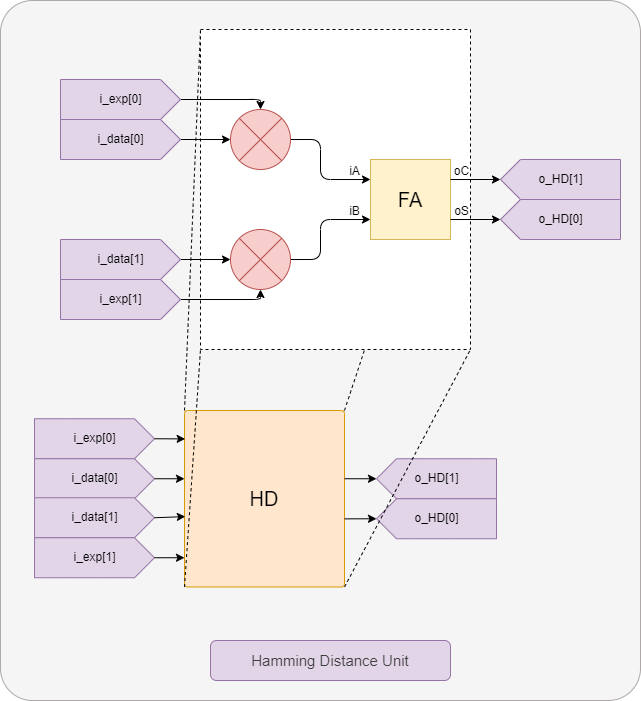
\includegraphics[width=.8\linewidth]{sections/pic/mophongbangSystemVerilog/HD_unit.png}
	\caption{Bộ tính toán khoảng cách Hamming.}
\end{figure}

\begin{figure}[H]
	\centering
	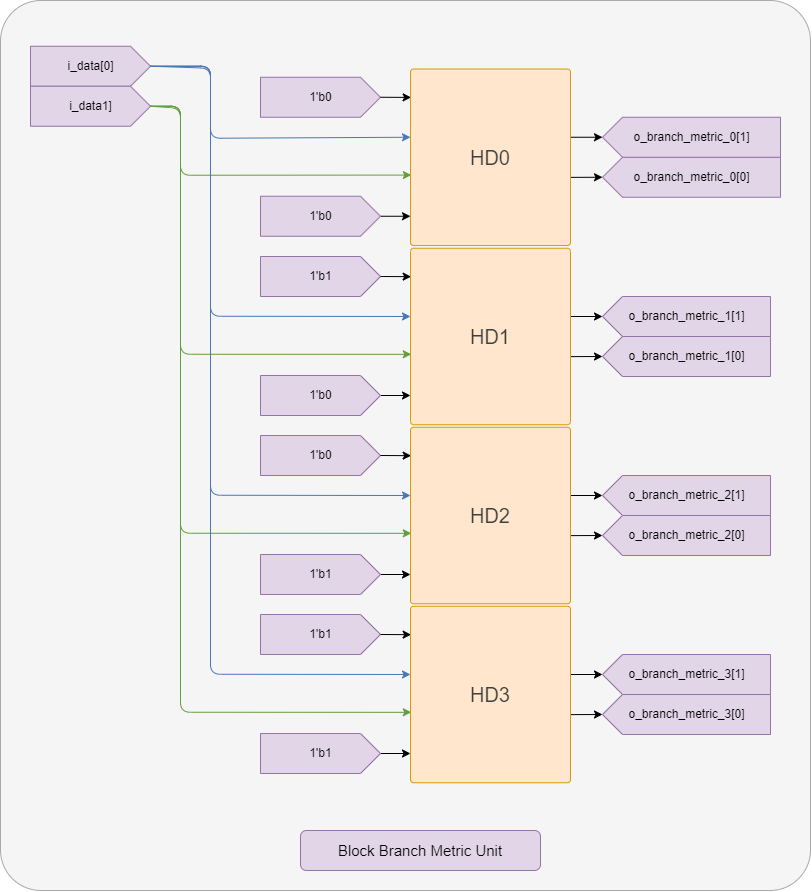
\includegraphics[width=.8\linewidth]{sections/pic/mophongbangSystemVerilog/BM_unit.png}
	\caption{Bộ BMU.}
\end{figure}

\begin{lstlisting}[style=StyleResult, language=Result]
	Time: 0 | i_rst_n = 0 | i_data: 00 | o_BM_0: 00 | o_BM_1: 00 | o_BM_2: 00 | o_BM_3: 00 | o_valid: 0
	Time: 5000 | i_rst_n = 0 | i_data: 00 | o_BM_0: 00 | o_BM_1: 00 | o_BM_2: 00 | o_BM_3: 00 | o_valid: 0
	Time: 5000 | i_rst_n = 0 | i_data: 00 | o_BM_0: 00 | o_BM_1: 00 | o_BM_2: 00 | o_BM_3: 00 | o_valid: 0
	Time: 5000 | i_rst_n = 0 | i_data: 00 | o_BM_0: 00 | o_BM_1: 00 | o_BM_2: 00 | o_BM_3: 00 | o_valid: 0
	Time: 10000 | i_rst_n = 1 | i_data: 00 | o_BM_0: 00 | o_BM_1: 00 | o_BM_2: 00 | o_BM_3: 00 | o_valid: 0
	Time: 10000 | i_rst_n = 1 | i_data: 00 | o_BM_0: 00 | o_BM_1: 00 | o_BM_2: 00 | o_BM_3: 00 | o_valid: 0
	Time: 15000 | i_rst_n = 1 | i_data: 00 | o_BM_0: 00 | o_BM_1: 00 | o_BM_2: 00 | o_BM_3: 00 | o_valid: 0
	Time: 15000 | i_rst_n = 1 | i_data: 00 | o_BM_0: 00 | o_BM_1: 00 | o_BM_2: 00 | o_BM_3: 00 | o_valid: 0
	Time: 15000 | i_rst_n = 1 | i_data: 00 | o_BM_0: 00 | o_BM_1: 01 | o_BM_2: 01 | o_BM_3: 10 | o_valid: 1
	Time: 20000 | i_rst_n = 1 | i_data: 00 | o_BM_0: 00 | o_BM_1: 01 | o_BM_2: 01 | o_BM_3: 10 | o_valid: 1
	Time: 20000 | i_rst_n = 1 | i_data: 00 | o_BM_0: 00 | o_BM_1: 01 | o_BM_2: 01 | o_BM_3: 10 | o_valid: 1
	Time: 25000 | i_rst_n = 1 | i_data: 00 | o_BM_0: 00 | o_BM_1: 01 | o_BM_2: 01 | o_BM_3: 10 | o_valid: 1
	Time: 25000 | i_rst_n = 1 | i_data: 00 | o_BM_0: 00 | o_BM_1: 01 | o_BM_2: 01 | o_BM_3: 10 | o_valid: 1
	Time: 25000 | i_rst_n = 1 | i_data: 00 | o_BM_0: 00 | o_BM_1: 01 | o_BM_2: 01 | o_BM_3: 10 | o_valid: 1
	Time: 30000 | i_rst_n = 1 | i_data: 00 | o_BM_0: 00 | o_BM_1: 01 | o_BM_2: 01 | o_BM_3: 10 | o_valid: 1
	Time: 30000 | i_rst_n = 1 | i_data: 00 | o_BM_0: 00 | o_BM_1: 01 | o_BM_2: 01 | o_BM_3: 10 | o_valid: 1
	Time: 35000 | i_rst_n = 1 | i_data: 00 | o_BM_0: 00 | o_BM_1: 01 | o_BM_2: 01 | o_BM_3: 10 | o_valid: 1
	Time: 35000 | i_rst_n = 1 | i_data: 01 | o_BM_0: 00 | o_BM_1: 01 | o_BM_2: 01 | o_BM_3: 10 | o_valid: 1
	Time: 35000 | i_rst_n = 1 | i_data: 01 | o_BM_0: 01 | o_BM_1: 00 | o_BM_2: 10 | o_BM_3: 01 | o_valid: 1
	Time: 40000 | i_rst_n = 1 | i_data: 01 | o_BM_0: 01 | o_BM_1: 00 | o_BM_2: 10 | o_BM_3: 01 | o_valid: 1
	Time: 40000 | i_rst_n = 1 | i_data: 01 | o_BM_0: 01 | o_BM_1: 00 | o_BM_2: 10 | o_BM_3: 01 | o_valid: 1
	Time: 45000 | i_rst_n = 1 | i_data: 01 | o_BM_0: 01 | o_BM_1: 00 | o_BM_2: 10 | o_BM_3: 01 | o_valid: 1
	Time: 45000 | i_rst_n = 1 | i_data: 01 | o_BM_0: 01 | o_BM_1: 00 | o_BM_2: 10 | o_BM_3: 01 | o_valid: 1
	Time: 45000 | i_rst_n = 1 | i_data: 01 | o_BM_0: 01 | o_BM_1: 00 | o_BM_2: 10 | o_BM_3: 01 | o_valid: 1
	Time: 50000 | i_rst_n = 1 | i_data: 01 | o_BM_0: 01 | o_BM_1: 00 | o_BM_2: 10 | o_BM_3: 01 | o_valid: 1
	Time: 50000 | i_rst_n = 1 | i_data: 01 | o_BM_0: 01 | o_BM_1: 00 | o_BM_2: 10 | o_BM_3: 01 | o_valid: 1
	Time: 55000 | i_rst_n = 1 | i_data: 01 | o_BM_0: 01 | o_BM_1: 00 | o_BM_2: 10 | o_BM_3: 01 | o_valid: 1
	Time: 55000 | i_rst_n = 1 | i_data: 10 | o_BM_0: 01 | o_BM_1: 00 | o_BM_2: 10 | o_BM_3: 01 | o_valid: 1
	Time: 55000 | i_rst_n = 1 | i_data: 10 | o_BM_0: 01 | o_BM_1: 10 | o_BM_2: 00 | o_BM_3: 01 | o_valid: 1
	Time: 60000 | i_rst_n = 1 | i_data: 10 | o_BM_0: 01 | o_BM_1: 10 | o_BM_2: 00 | o_BM_3: 01 | o_valid: 1
	Time: 60000 | i_rst_n = 1 | i_data: 10 | o_BM_0: 01 | o_BM_1: 10 | o_BM_2: 00 | o_BM_3: 01 | o_valid: 1
	Time: 65000 | i_rst_n = 1 | i_data: 10 | o_BM_0: 01 | o_BM_1: 10 | o_BM_2: 00 | o_BM_3: 01 | o_valid: 1
	Time: 65000 | i_rst_n = 1 | i_data: 10 | o_BM_0: 01 | o_BM_1: 10 | o_BM_2: 00 | o_BM_3: 01 | o_valid: 1
	Time: 65000 | i_rst_n = 1 | i_data: 10 | o_BM_0: 01 | o_BM_1: 10 | o_BM_2: 00 | o_BM_3: 01 | o_valid: 1
	Time: 70000 | i_rst_n = 1 | i_data: 10 | o_BM_0: 01 | o_BM_1: 10 | o_BM_2: 00 | o_BM_3: 01 | o_valid: 1
	Time: 70000 | i_rst_n = 1 | i_data: 10 | o_BM_0: 01 | o_BM_1: 10 | o_BM_2: 00 | o_BM_3: 01 | o_valid: 1
	Time: 75000 | i_rst_n = 1 | i_data: 10 | o_BM_0: 01 | o_BM_1: 10 | o_BM_2: 00 | o_BM_3: 01 | o_valid: 1
	Time: 75000 | i_rst_n = 1 | i_data: 11 | o_BM_0: 01 | o_BM_1: 10 | o_BM_2: 00 | o_BM_3: 01 | o_valid: 1
	Time: 75000 | i_rst_n = 1 | i_data: 11 | o_BM_0: 10 | o_BM_1: 01 | o_BM_2: 01 | o_BM_3: 00 | o_valid: 1
	Time: 80000 | i_rst_n = 1 | i_data: 11 | o_BM_0: 10 | o_BM_1: 01 | o_BM_2: 01 | o_BM_3: 00 | o_valid: 1
	Time: 80000 | i_rst_n = 1 | i_data: 11 | o_BM_0: 10 | o_BM_1: 01 | o_BM_2: 01 | o_BM_3: 00 | o_valid: 1
	Time: 85000 | i_rst_n = 1 | i_data: 11 | o_BM_0: 10 | o_BM_1: 01 | o_BM_2: 01 | o_BM_3: 00 | o_valid: 1
	Time: 85000 | i_rst_n = 1 | i_data: 11 | o_BM_0: 10 | o_BM_1: 01 | o_BM_2: 01 | o_BM_3: 00 | o_valid: 1
	Time: 85000 | i_rst_n = 1 | i_data: 11 | o_BM_0: 10 | o_BM_1: 01 | o_BM_2: 01 | o_BM_3: 00 | o_valid: 1
	Time: 90000 | i_rst_n = 1 | i_data: 11 | o_BM_0: 10 | o_BM_1: 01 | o_BM_2: 01 | o_BM_3: 00 | o_valid: 1
	Time: 90000 | i_rst_n = 1 | i_data: 11 | o_BM_0: 10 | o_BM_1: 01 | o_BM_2: 01 | o_BM_3: 00 | o_valid: 1
	Time: 95000 | i_rst_n = 1 | i_data: 11 | o_BM_0: 10 | o_BM_1: 01 | o_BM_2: 01 | o_BM_3: 00 | o_valid: 1
	Time: 95000 | i_rst_n = 1 | i_data: 11 | o_BM_0: 10 | o_BM_1: 01 | o_BM_2: 01 | o_BM_3: 00 | o_valid: 1
	Time: 95000 | i_rst_n = 1 | i_data: 11 | o_BM_0: 10 | o_BM_1: 01 | o_BM_2: 01 | o_BM_3: 00 | o_valid: 1
	- tb_bmu.sv:53: Verilog $finish
	Time: 100000 | i_rst_n = 1 | i_data: 11 | o_BM_0: 10 | o_BM_1: 01 | o_BM_2: 01 | o_BM_3: 00 | o_valid: 1
	Time: 100000 | i_rst_n = 1 | i_data: 11 | o_BM_0: 10 | o_BM_1: 01 | o_BM_2: 01 | o_BM_3: 00 | o_valid: 	
\end{lstlisting}

\subsection{Add Compare Select Unit (ACSU)}

\begin{figure}[H]
	\centering
	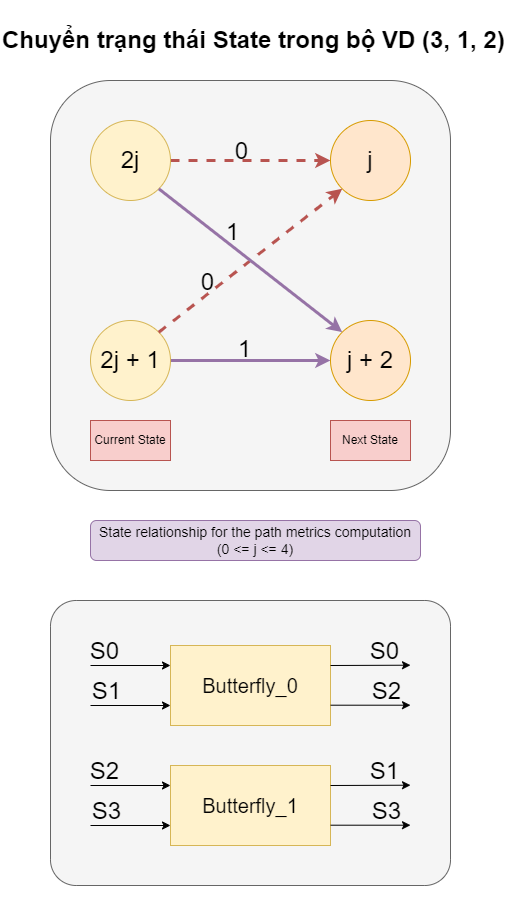
\includegraphics[width=.6\linewidth]{sections/pic/mophongbangSystemVerilog/ACSU_proc_state.png}
	\caption{Cách chuyển trạng thái trong bộ giải mã Viterbi ($3, 1, 2$).}
\end{figure}

\begin{figure}[H]
	\centering
	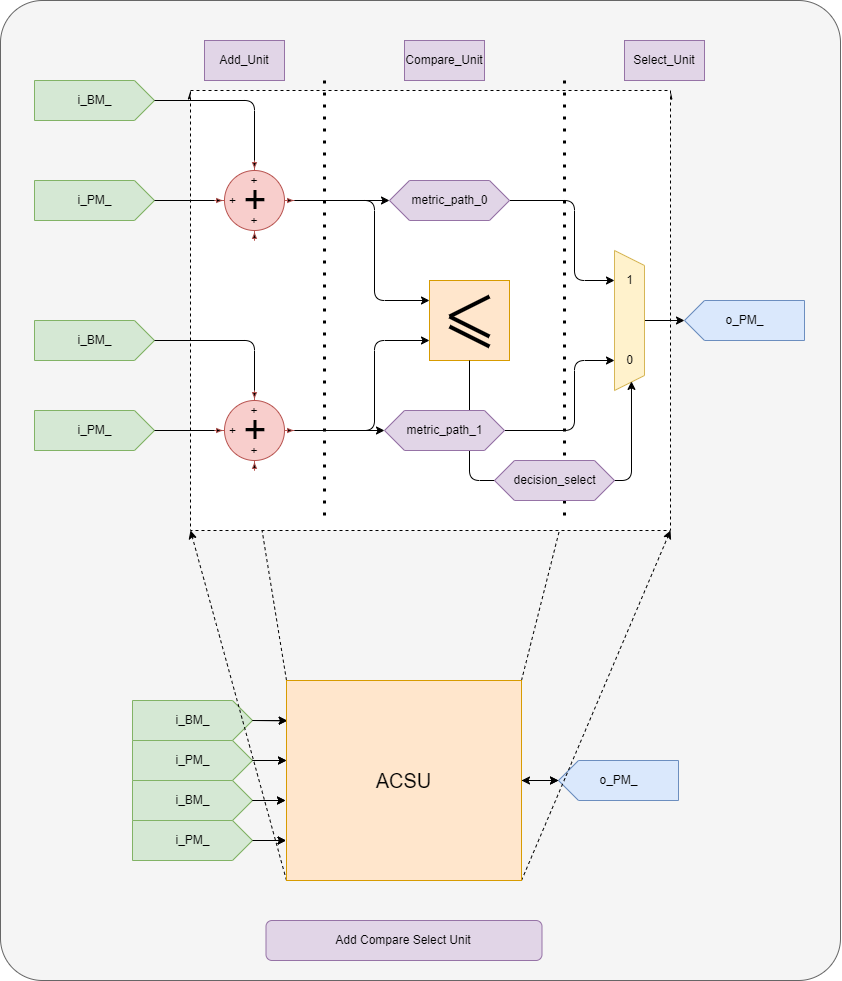
\includegraphics[width=.8\linewidth]{sections/pic/mophongbangSystemVerilog/ACS.png}
	\caption{Bộ Add Compare Select.}
\end{figure}

\begin{figure}[H]
	\centering
	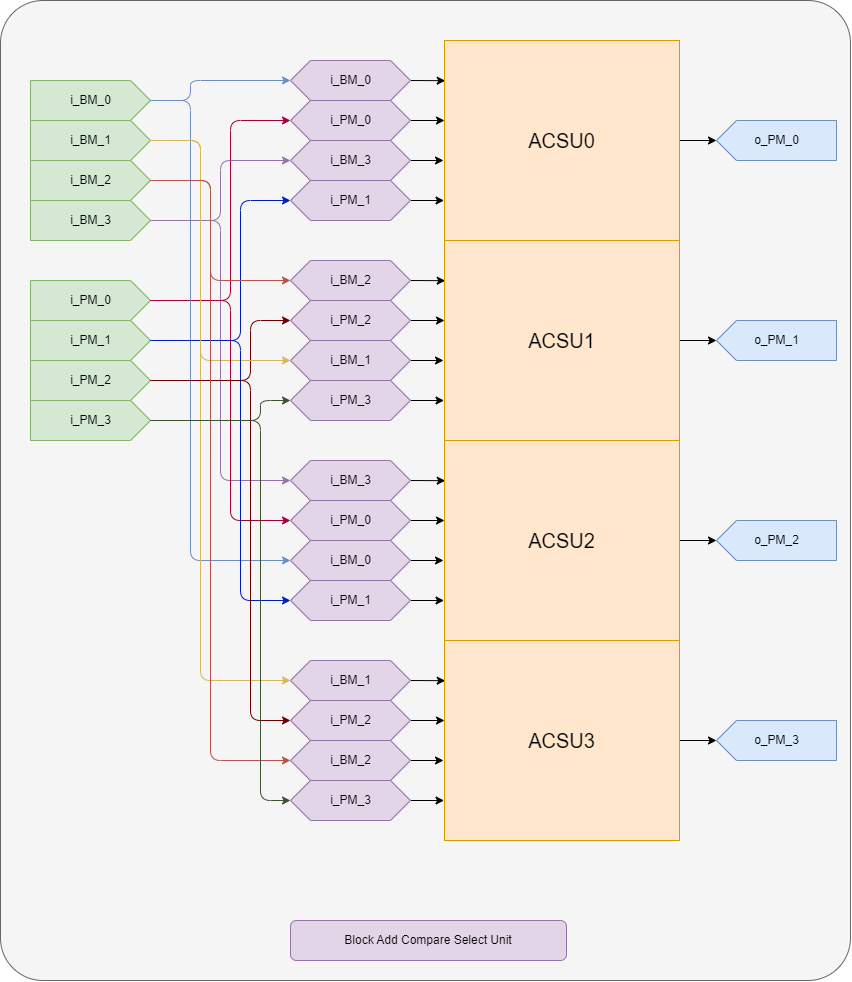
\includegraphics[width=.8\linewidth]{sections/pic/mophongbangSystemVerilog/ACSU.png}
	\caption{Bộ ACSU hoàn chỉnh.}
\end{figure}

\begin{lstlisting}[style=StyleResult, language=Result]
	Starting Add_unit testbench...
	============================
	Time: 0 | i_rst_n = 0 | 
	| i_BM_0: 00 | i_BM_1: 00 | i_BM_2: 00 | i_BM_3: 00 |
	| i_iPM_0: 00 | i_iPM_1: 00 | i_iPM_2: 00 | i_iPM_3: 00 |
	| o_oPM_0: 00 | o_oPM_1: 00 | o_oPM_2: 00 | o_oPM_3: 00
	Time: 10000 | i_rst_n = 1 | 
	| i_BM_0: 00 | i_BM_1: 00 | i_BM_2: 00 | i_BM_3: 00 |
	| i_iPM_0: 00 | i_iPM_1: 11 | i_iPM_2: 11 | i_iPM_3: 11 |
	| o_oPM_0: 00 | o_oPM_1: 00 | o_oPM_2: 00 | o_oPM_3: 00
	Time: 25000 | i_rst_n = 1 | 
	| i_BM_0: 00 | i_BM_1: 00 | i_BM_2: 10 | i_BM_3: 00 |
	| i_iPM_0: 00 | i_iPM_1: 00 | i_iPM_2: 00 | i_iPM_3: 00 |
	| o_oPM_0: 00 | o_oPM_1: 00 | o_oPM_2: 00 | o_oPM_3: 00
	Time: 35000 | i_rst_n = 1 | 
	| i_BM_0: 00 | i_BM_1: 00 | i_BM_2: 10 | i_BM_3: 00 |
	| i_iPM_0: 00 | i_iPM_1: 00 | i_iPM_2: 00 | i_iPM_3: 00 |
	| o_oPM_0: 00 | o_oPM_1: 00 | o_oPM_2: 00 | o_oPM_3: 00
	Time: 45000 | i_rst_n = 1 | 
	| i_BM_0: 11 | i_BM_1: 11 | i_BM_2: 01 | i_BM_3: 01 |
	| i_iPM_0: 00 | i_iPM_1: 00 | i_iPM_2: 00 | i_iPM_3: 00 |
	| o_oPM_0: 00 | o_oPM_1: 00 | o_oPM_2: 00 | o_oPM_3: 00
	Time: 55000 | i_rst_n = 1 | 
	| i_BM_0: 01 | i_BM_1: 10 | i_BM_2: 10 | i_BM_3: 01 |
	| i_iPM_0: 00 | i_iPM_1: 00 | i_iPM_2: 00 | i_iPM_3: 00 |
	| o_oPM_0: 01 | o_oPM_1: 01 | o_oPM_2: 01 | o_oPM_3: 01
	Time: 65000 | i_rst_n = 1 | 
	| i_BM_0: 10 | i_BM_1: 10 | i_BM_2: 01 | i_BM_3: 00 |
	| i_iPM_0: 01 | i_iPM_1: 01 | i_iPM_2: 01 | i_iPM_3: 01 |
	| o_oPM_0: 01 | o_oPM_1: 10 | o_oPM_2: 01 | o_oPM_3: 10
	Time: 75000 | i_rst_n = 1 | 
	| i_BM_0: 11 | i_BM_1: 00 | i_BM_2: 10 | i_BM_3: 00 |
	| i_iPM_0: 01 | i_iPM_1: 10 | i_iPM_2: 01 | i_iPM_3: 10 |
	| o_oPM_0: 00 | o_oPM_1: 01 | o_oPM_2: 00 | o_oPM_3: 01
	Time: 85000 | i_rst_n = 1 | 
	| i_BM_0: 10 | i_BM_1: 10 | i_BM_2: 10 | i_BM_3: 10 |
	| i_iPM_0: 00 | i_iPM_1: 01 | i_iPM_2: 00 | i_iPM_3: 01 |
	| o_oPM_0: 00 | o_oPM_1: 00 | o_oPM_2: 00 | o_oPM_3: 00
	Time: 95000 | i_rst_n = 1 | 
	| i_BM_0: 00 | i_BM_1: 10 | i_BM_2: 11 | i_BM_3: 00 |
	| i_iPM_0: 00 | i_iPM_1: 00 | i_iPM_2: 00 | i_iPM_3: 00 |
	| o_oPM_0: 10 | o_oPM_1: 10 | o_oPM_2: 10 | o_oPM_3: 10
	Time: 105000 | i_rst_n = 1 | 
	| i_BM_0: 01 | i_BM_1: 10 | i_BM_2: 10 | i_BM_3: 01 |
	| i_iPM_0: 10 | i_iPM_1: 10 | i_iPM_2: 10 | i_iPM_3: 10 |
	| o_oPM_0: 00 | o_oPM_1: 10 | o_oPM_2: 00 | o_oPM_3: 10
	Time: 115000 | i_rst_n = 1 | 
	| i_BM_0: 11 | i_BM_1: 00 | i_BM_2: 11 | i_BM_3: 10 |
	| i_iPM_0: 00 | i_iPM_1: 10 | i_iPM_2: 00 | i_iPM_3: 10 |
	| o_oPM_0: 01 | o_oPM_1: 10 | o_oPM_2: 01 | o_oPM_3: 10
	Time: 125000 | i_rst_n = 1 | 
	| i_BM_0: 11 | i_BM_1: 01 | i_BM_2: 10 | i_BM_3: 11 |
	| i_iPM_0: 01 | i_iPM_1: 10 | i_iPM_2: 01 | i_iPM_3: 10 |
	| o_oPM_0: 10 | o_oPM_1: 00 | o_oPM_2: 10 | o_oPM_3: 00
	Simulation finished.
	==================================
	- tb_acsu.sv:80: Verilog $finish
\end{lstlisting}

\subsection{Survivor Path Memory Unit (SPMU)}

\begin{figure}[H]
	\centering
	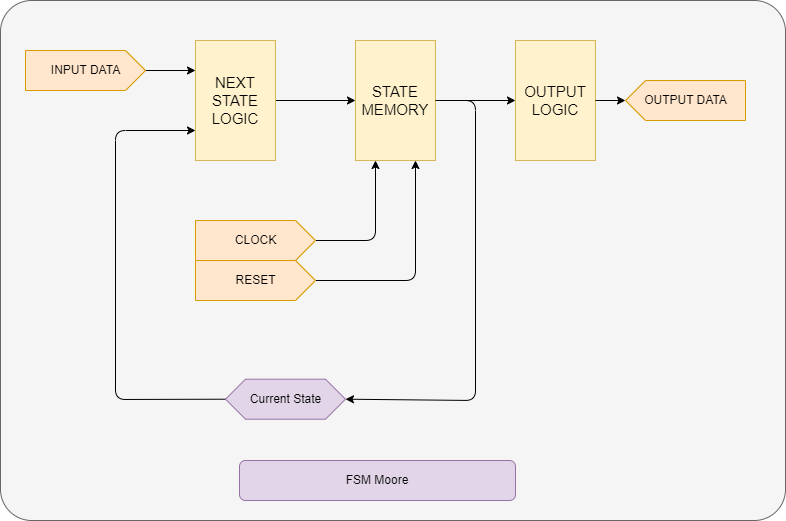
\includegraphics[width=.8\linewidth]{sections/pic/mophongbangSystemVerilog/FSM.png}
	\caption{Máy trạng thái viết ở dạng Moore.}
\end{figure}

\begin{figure}[H]
	\centering
	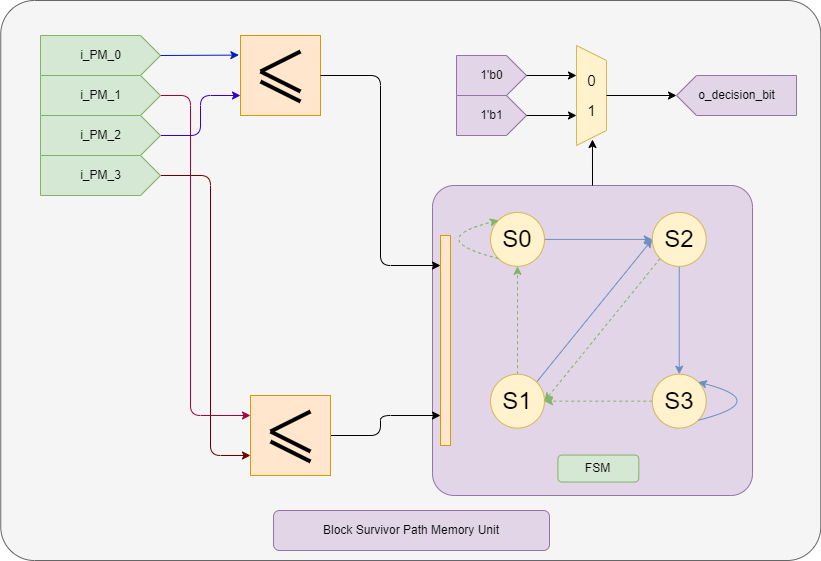
\includegraphics[width=.8\linewidth]{sections/pic/mophongbangSystemVerilog/SPMU.png}
	\caption{Bộ SPMU.}
\end{figure}

\begin{lstlisting}[style=StyleResult, language=Result]
	Time =                 5000 	| i_rst_n = 1 	| o_decision = 0 	| o_valid = 0 	|
	PM_0 = 0 	| PM_1 = 0 	| PM_2 = 0 	| PM_3 = 0 	| 
	=========================================
	case 1: S0 -> S0
	Time = 15000 	| i_rst_n = 1 	| o_decision = 0 	| o_valid = 1 	|
	PM_0 = 0 	| PM_1 = 1 	| PM_2 = 2 	| PM_3 = 3 	| 
	=========================================
	case 2: S0 -> S2
	Time = 25000 	| i_rst_n = 1 	| o_decision = 0 	| o_valid = 1 	|
	PM_0 = 3 	| PM_1 = 2 	| PM_2 = 1 	| PM_3 = 0 	| 
	=========================================
	case 3: S2 -> S1
	Time = 35000 	| i_rst_n = 1 	| o_decision = 1 	| o_valid = 1 	|
	PM_0 = 2 	| PM_1 = 0 	| PM_2 = 0 	| PM_3 = 1 	| 
	=========================================
	case 4: S1 -> S2
	Time = 45000 	| i_rst_n = 1 	| o_decision = 1 	| o_valid = 1 	|
	PM_0 = 3 	| PM_1 = 0 	| PM_2 = 1 	| PM_3 = 2 	| 
	=========================================
	case 5: S2 -> S3
	Time = 55000 	| i_rst_n = 1 	| o_decision = 0 	| o_valid = 1 	|
	PM_0 = 1 	| PM_1 = 2 	| PM_2 = 3 	| PM_3 = 0 	| 
	=========================================
	case 6: S3 -> S3
	Time = 65000 	| i_rst_n = 1 	| o_decision = 1 	| o_valid = 1 	|
	PM_0 = 3 	| PM_1 = 2 	| PM_2 = 1 	| PM_3 = 0 	| 
	=========================================
	Testbench completed successfully
	==================================
	- tb_spmu.sv:113: Verilog $finish
\end{lstlisting}